\documentclass[review,12pt]{elsarticle}

\usepackage{amsmath} % for mathematical symbols and formulas
\usepackage{amssymb} % for mathematical symbols
\usepackage{graphicx} % for including graphics
\usepackage{hyperref} % for hyperlinks
\usepackage{booktabs}

\makeatletter
\def\ps@pprintTitle{%
    \let\@oddhead\@empty
    \let\@evenhead\@empty
    \def\@oddfoot{\hfill December 2024} % Keeps the date in the footer
    \let\@evenfoot\@oddfoot
}
\makeatother


\begin{document}

\title {Thesis Report \\[1ex] \large The use of generative deep learning to synthesize realistic healthcare digital twins}
\author {Laura Jochim}


\maketitle


\section{ Introduction}
A recent development within the research field of medicine is the creation of a more holistic approach and the targeting of person-specific treatments. One relatively new approach to achieving a holistic medical research field is the creation of digital twins. A digital twin is a virtual replica of a real human patient \cite{jpm13101522}. Digital twins can help clinicians to gain valuable insights, optimize treatment strategies, and deliver personalized care. Furthermore, the application of digital twins can help reduce animal testing, ensure privacy when sharing data, and address ethical concerns during data collection \cite{Subramanian2020DigitalTF}. Even though the use of digital twins within the healthcare sector is a relatively new development, it is known to be a promising tool to virtually replicate human body parts or create data-driven digital twins \cite{GILLETTE2021102080}, \cite{KOVATCHEV2019432}. \\
Such a digital twin is created on the basis of synthetic data, i.e., fake data that resembles real-world data. The idea of synthetic data was initially proposed by Rubin \cite{scb2023disclosure}, where he suggested drawing synthetic samples using a multiple imputation approach to handle missing data \cite{MR742974}, \cite{Rubin2002MULTIPLEII}, similar to what is implemented in R by mice \cite{mice}. In the following years, advanced, machine learning, techniques have been incorporated to account for complex sampling designs \cite{10.1214/24-STS927}. The computer science field also started to develop approaches, many were developed around 2014. Examples are Bayesian networks \cite{bayesian_network}, copulas \cite{article}, and generative adversarial networks (GANs) \cite{goodfellow2014generativeadversarialnetworks}. Especially GANs resulted in a boost in synthetic data research and applications in the computer science literature \cite{10.1214/24-STS927}. 
\\
This project will focus on GANs to synthesize digital twins. GANs have been widely used in several fields to generate images and sound data. In healthcare, a recent increase in the popularity of GANs has been seen, showing good performance in literature especially because of their flexibility \cite{AGGARWAL2021100004}. Briefly, a GAN is a neural network involving a generator and a discriminator \cite{goodfellow2014generativeadversarialnetworks}. The generator produces synthetic samples and is finetuned through the discriminator to generate data matching the training data characteristics. An example of how the GAN generates data that increasingly resembles training data is shown in Figure 1.
\begin{figure} [hbt!]
    \centering
    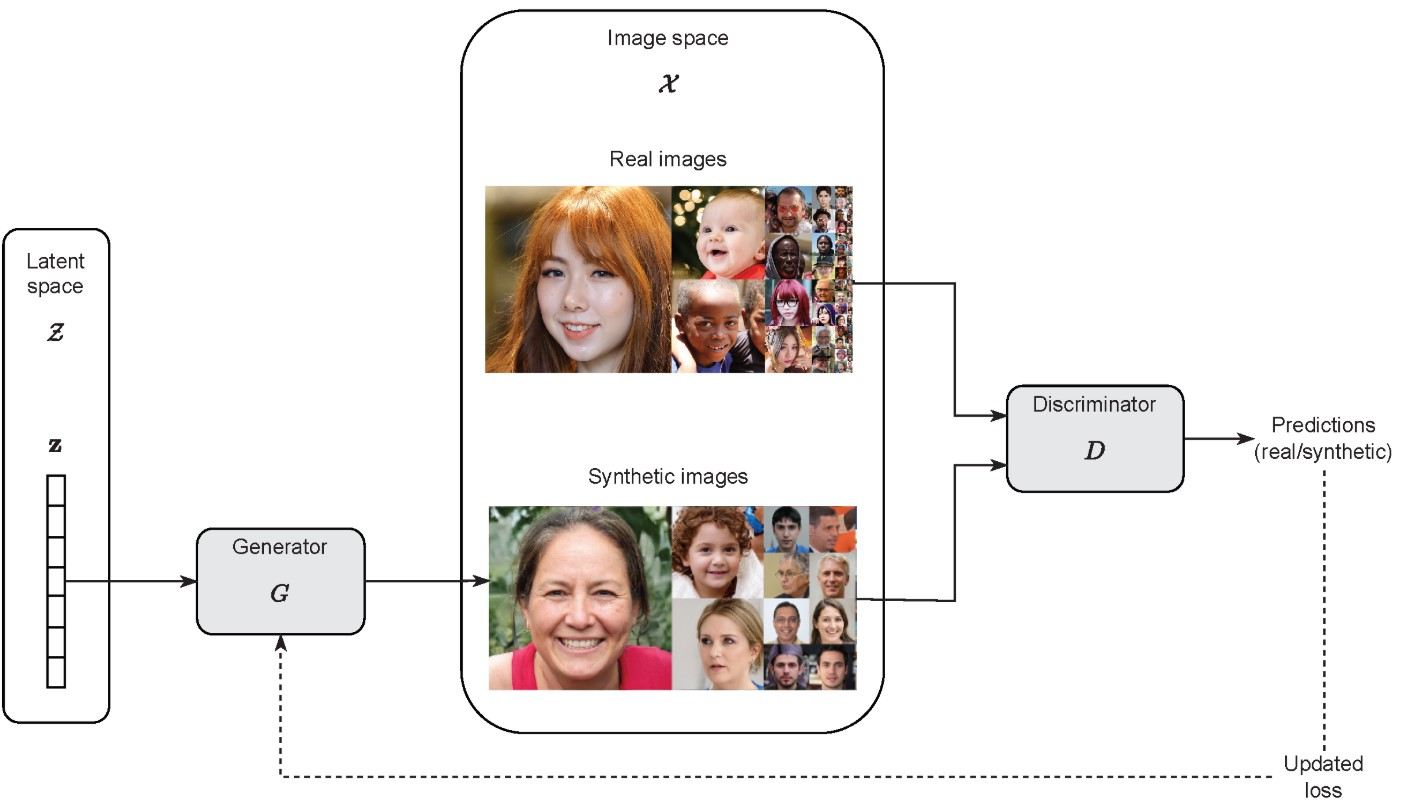
\includegraphics[width=1\linewidth]{Screenshot 2024-12-18 145130.jpg}
    \caption{A visual example of how a GAN works with imaging data \cite{app13020816}. The discriminator is presented with both real and synthetic images of faces where the synthetic images are generated from a latent space $Z$. The discriminator's decision (real/fake) is used to update the loss of the generator which in return tries to produce more realistic looking images iteratively. 
}
    \label{
}
\end{figure} % https://www.mdpi.com/2076-3417/13/2/816
GANs are usually used for image data, as seen in Figure 1, though healthcare data is often represented in a table, where rows represent the patient and columns the patient's characteristics. The problems GANs often face when dealing with this kind of tabular data include (1) simultaneously modeling continuous and discrete variables, (2) the columns with complicated distributions, often a mixture of non-Gaussian  distributions, and (3) the severe imbalance of categories within a column (over- or underrepresentation of a category) \cite{xu2019modelingtabulardatausing}. To deal with these issues the conditional tabular GAN (ctGAN) \cite{DBLP:journals/corr/abs-1907-00503} has been developed which will be used for this project.\\
Another characteristic of healthcare data is that it usually has a rather small sample size, which could lead to problems. Deep learning methods like GANs typically require a large sample size to train on to prevent over- and undersampling of specific data characteristics. GANs may also be prone to overfit when only a small sample size is available. Efforts have been made to include prior knowledge in the training phase to reduce overfitting \cite{10.1093/bioinformatics/btab608}. Therefore, the aim is to implement prior knowledge in the flexible ctGAN structure and evaluate whether this works within the healthcare field. The research questions of this project are: To what extent are ctGANs applicable given the challenges of small sample-sized healthcare data? Specifically, will including prior knowledge in the ctGAN framework lead to more realistic digital twins even when the sample size is limited?


\section{ Methodology}
The workflow of this paper is based on the ctGAN architecture \cite{ctgan} with modifications necessary to deal with healthcare data. In this section, we will give an overview of what a neural network is, how a GAN works, and how the ctGAN architecture handles issues encountered with healthcare data, that the GAN architecture struggles with. Lastly, we will elaborate on how to evaluate the ctGAN's performance. \\


\subsection{Neural Networks} 
A GAN consists of two neural networks, so it is important to introduce what a neural network is. A neural network is a non-linear mapping that consists of one or more layers of latent (or hidden) variables. The input layer consists of the data variables while the subsequent layers consist of variables that are non-linear transformations of the output of the previous layer. These transformations are generally constructed by a linear transformation, including an intercept, of the previous variables and a non-linear activation function. For example, a particular latent variable in a hidden layer can be written as $f(x) = \varphi(x^\top w + b)$. Some often chosen activation functions are a rectified linear unit (RELU) and a sigmoid. The output $y$ is then modeled in terms of $x$ via a chain of activation functions and linear transformations, e.g. $y = f_1(f_2(f_3(x)))$ for three hidden layers. The parameters that are estimated during training are the weights $w$ and intercepts $b$ from each layer. To optimize these parameters, numerical optimization techniques are used that are implemented in Python deep learning libraries such as PyTorch \cite{NEURIPS2019_9015}. 
\\

\subsection{Generative Adversarial Network}
The GAN framework, introduced by Ian Goodfellow et al. \cite{goodfellow2014generativeadversarialnetworks}, consists of two competing neural networks: a generator and a discriminator, which are trained simultaneously in a game-theoretic setup; see Figure 1. 
\\%%%% Maybe here?
The generator transforms samples from random input $z$ sampled from a prior distribution ($p_z(z)$), typically uniform or Gaussian, to a data space aiming to obtain realistic data samples by capturing the data distribution. The discriminator takes an input $x$ and outputs $y$, which is a binary outcome, indicating whether the input comes from generated or real data ($p_{data}(x)$). Then the discriminator’s evaluation ("fake"/"real") is used to compute the generator’s loss, which is then minimized through backpropagation, updating the generator's weights to improve its performance. 
\\The idea is to train the generator enough iterations that it starts producing output resembling the training data and ‘fool’ the discriminator into classifying the generated data as real. In theory, the training is completed when the discriminator cannot tell generated and real data apart and therefore has a probability of 0.5, i.e., random classification. This minmax game can be written as a value function,
\\
\\
\begin{equation} 
\min_G \max_D V(G, D) = \mathbb{E}_{x \sim p_{\text{data}}(x)} \left[ \log D(x) \right] + \mathbb{E}_{z \sim p_z(z)} \left[ \log \left( 1 - D(G(z)) \right) \right],
\end{equation}
\\
\\
where $G$ annotates the generator and $D$ the discriminator. The first term trains the discriminator to maximize the probability of identifying the real data, ideally close to 1, whereas the second term trains the discriminator to minimize the probability of identifying the fake data from the generator as real, ideally close to 0. 
Note that for a well-trained discriminator, $D(x$) is close to 1 and $D(G(z))$ is close to zero, maximizing the combined score $V$. And for a well-trained generator, the $D(G(z))$ is close to 1, which worsens the performance of the discriminator.
Once conversion is reached and the GAN is trained to produce real-looking data, one can use the trained generator to obtain synthesized data. 
\\
\subsection{CTGAN}
For this project it is especially interesting to look at the ctGAN architecture, a GAN designed for tabular data, which has been shown to outperform alternative architectures for tabular data \cite{xu2019modelingtabulardatausing}. The GAN structure is most often used for image data and is therefore useful in e.g., medical imaging. This project will deal with medical tabular data, where each patient is listed in a row with columns representing clinical data e.g., patient demographic, information about mutated genes, and cancer tumor stage. The problems GANs usually run into when dealing with tabular data were addressed using the ctGAN \cite{DBLP:journals/corr/abs-1907-00503}, see Figure 2. 
\begin{figure} [hbt!]
    \centering
    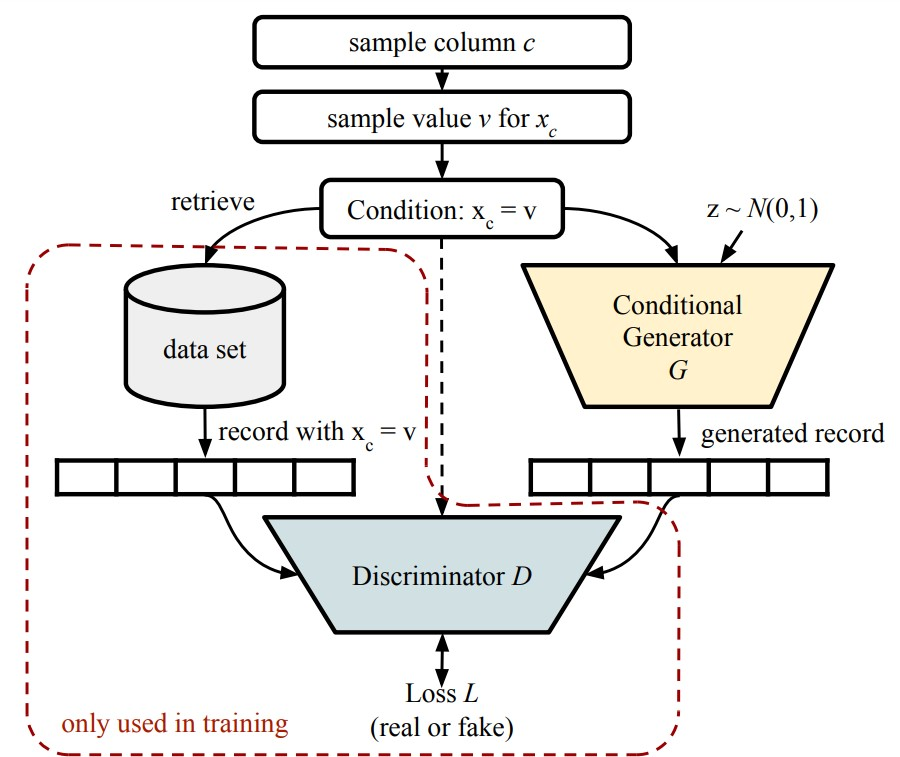
\includegraphics[width=80mm,scale=0.5]{Screenshot 2024-12-18 143855.jpg}
    \caption{For the ctGAN \cite{DBLP:journals/corr/abs-2110-01889}, the generator has a condition term. First, a column and then a value of said column is sampled. This condition $x_c = v$ and noise $z \sim \mathcal{N}(0, 1)$ is fed into the generator $G$ to produce a synthetic record that adheres to the condition. Both the real record (retrieved from the dataset) and the generated record are passed to the Discriminator $D$. The Loss $L$, calculated based on the discriminator's output, is used to update both the generator and discriminator during training.
  }
    \label{
}
\end{figure}
\\ To overcome the issue of modeling non-Gaussian and multimodal distribution, i.e. columns with complicated distribution, the developers of ctGAN invented mode-specific normalization \cite{xu2019modelingtabulardatausing}. In this method, each column is processed independently in three steps. For each column, the number of modes is estimated and a Gaussian mixture \cite{bishop2006pattern} is fitted. Then for each value in the column, its membership probability for each of the mixture distributions is computed. 
%Lastly, one mode is sampled from the probability density, and the sampled mode is used to normalize the value. 
Lastly, the values are then z-transformed with respect to one of the mixture distributions using the estimated mean and variance of that Gaussian distribution. 
Note, that to capture the full diversity of the data’s distribution, mode-specific normalization is dynamically applied throughout the training process. Instead of the usual normalizing in the preprocessing stage, the generator can adapt to the data’s structure and conditional dependencies throughout the training.\\ 
To address the issue of imbalanced categorical variables ctGAN implements a conditional generator and training-by-sampling. The generator is conditioned to focus on specific categories, mainly less represented categories, during the learning process to be able to create more realistic data even when training data is limited. The loss function includes a penalty for the generator when its output does not match the desired category. This penalty ensures that the generator learns to produce data that aligns with the given conditions, making its outputs more accurate.\\ At the same time, training-by-sampling ensures that the final data reflects the real distribution by avoiding bias through over- or undersampling. This is done by sampling based on the log-frequency of each category. It ensures that less frequent categories are given more representation during training without distorting the overall data distribution. 
\\
To incorporate prior knowledge in the ctGAN architecture a regularization term $R(G)$ is introduced which is weighted by the hyperparameter $\lambda$ modifying the loss functions as follows:
\\
\\
\begin{equation} \label{eu_eqn}
\min_G \max_D (V(G, D + \lambda R(G))
\end{equation}
\\
\\
The loss function governs how both components, generator and discriminator, improve over time. Including a regularization term aids in implementing prior knowledge by introducing constraints. A penalty can be imposed to reflect the prior knowledge that certain features should (not) be correlated. The neural network architecture underlying the generator $G$ will then be penalized towards (or away from) inducing correlations between these features. Following the three-stage method developed by Anderson, Gadgil, Johnson, Schwab, and Davidson (2021) \cite{ANDERSON2021104850}, the inclusion of prior knowledge can be achieved by combining it with the output of the final layer of the neural network. In the thesis, we will further explore possible ways to incorporate prior knowledge where available. 
%%%% Maybe add: min max V(G,D) + \lambda Pen(G,D)
\\
\\
\subsection{Data and Software Description}
The data used for this project is the following freely accessible and comprehensive datasets: the TCGA Breast Cancer (BRCA) dataset from cBioPortal \cite{lingle2016tcgabrca} and the 10,000-Patient Database from Figshare \cite{Kartoun2018}. The BRCA dataset, with a sample size of 1101, provides detailed clinical and molecular data for breast cancer patients. We consider demographics, treatment history, cancer subtypes, proteomics, and genomics data. 
%%% number of features of the proteomics+genomics. and number of cancer subtypes
\\

\begin{table}[h!]
\centering
\caption{A virtual patient repository of 10,000 patients.}
\begin{tabular}{@{}lp{8cm}r@{}}
\toprule
\textbf{Variable and category} & \textbf{Patients} \\
\textbf{} & \textbf{(n = 10,000)} \\ 
\midrule
Mean age as of 1/1/2015, years (SD) & 57.8 (17.3) \\ 
Gender (\%) & \\
\hspace{1em} Female & 52.0 \\ 
Ethnicity (\%) & \\
\hspace{1em} White & 49.0 \\ 
\hspace{1em} Asian & 23.0 \\ 
\hspace{1em} African American & 15.0 \\ 
\hspace{1em} Unknown & 13.0 \\ 
Mean number of admissions per patient (SD) & 3.6 (1.5) \\ 
Mean length of stay, days (SD) & 11.0 (5.2) \\ 
\% Population with length of follow-up (years) & \\ 
\hspace{1em} 0–9 & 13.1 \\ 
\hspace{1em} 10–15 & 9.3 \\ 
\hspace{1em} \textgreater 15 & 77.6 \\ 
Population below poverty (\%) & 21.6 \\ 
Comorbidities; Prevalence (\%) & \\ 
\hspace{1em} Malignant neoplasm & 41.4 \\ 
\hspace{1em} Rheumatoid arthritis & 25.6 \\ 
\hspace{1em} Diabetes (type I or II) & 24.4 \\ 
\hspace{1em} Renal complications & 17.0 \\ 
\hspace{1em} Coronary artery disease & 7.0 \\ 
Laboratory values (Mean; SD) & \\ 
\hspace{1em} Blood urea nitrogen (mg/dL) & 17.5; 7.2 \\ 
\hspace{1em} Platelets (k/cumm) & 284.9; 95.3 \\ 
\hspace{1em} Creatinine (mg/dL) & 0.9; 0.2 \\ 
\hspace{1em} Albumin (gm/dL) & 4.2; 1.0 \\ 
\hspace{1em} Lymphocytes (\%) & 25; 5.8 \\ 
\bottomrule
\end{tabular}
\end{table}


The 10,000-Patient Database contains clinical and demographic information on virtual patients across various healthcare settings, with variables such as patient admission details, diagnoses, demographics, socioeconomic details, and approximately 50 diagnostic lab measurements, across multiple time points. 
\\
An interface to ctGAN is implemented in R and Python. We use the R package RCTGAN \cite{ctgan_r_package} for the first exploration stages in the software RStudio \cite{R}. Incorporating prior knowledge is performed in Pytorch \cite{NEURIPS2019_9015} either by implementing a custom generator and discriminator, or using the Python-CTGAN library \cite{SDV}.
\\
\subsection{Analysis plan}
To evaluate the GAN's performance the training-test-split procedure is applied. The common 80/20 split is used where the GAN is trained on 80 percent of the data. In the process of training a GAN different parameters are tuned, like the learning rate and the optimizer which will be explored during the project. Once convergence is reached, the generator is used to synthesize data. 
\\
To evaluate this newly obtained data on how realistic it is, the synthetic data is compared to the 20 percent test data. First, the distributions are compared on means, variances, skewness, and kurtosis. A permutation test is performed to test whether these quantities are different between real and synthetic data. Then we look at whether the correlations present in the real data are also present in the synthetic data. Here we plot a heatmap of the correlation to see where correlations tend to overlap. A few key variables are chosen to see whether their correlation is similar in the real and synthesized data. Lastly, the Kullback-Leibler divergence, which is the expected value of the log-likelihood ratio, is used to identify how dissimilar the probability distributions of the synthetic and real data are. A Kolmogorov-Smirnov test is then conducted to investigate whether the difference between the probability distributions of synthetic and real data is significantly different. Based on the information obtained, we decide whether the GAN is trained properly and performs well in synthesizing data.

 

\newpage
\bibliography{sources.bib}
\bibliographystyle{ieeetr}
\end{document}
